\documentclass[12pt]{article}
\input{../headers/assignment_header.tex}
\usepackage{aliascnt}
\usepackage{stmaryrd}
\usepackage{cancel}
\usepackage{booktabs}
\usepackage{floatrow}
\usepackage{caption}
\usepackage[nameinlink]{cleveref} % make \cref emulate look of \autoref

\crefname{thm}{Theorem}{Theorem}
\crefname{prop}{Proposition}{Proposition}
\crefname{cor}{Corollary}{Corollary}
\crefname{lem}{Lemma}{Lemma}
\crefname{dfn}{Definition}{Definition}
\betternewtcbtheorem[number within= section,use counter=thm]{thm}{Theorem}%
{
    breakable,
	enhanced,
	colback=green!10,
	colframe=green!35!black,
	fonttitle=\bfseries,
	top=3mm,
	attach boxed title to top left={xshift = 5mm, yshift=-1.5mm},
	boxed title style = {colback=green!35!black},
    title after break={},
    label type = thm
}{thm}
\betternewtcbtheorem[number within= section, use counter=thm]{dfn}{Definition}%
{
    breakable,
	enhanced,
	colback=blue!10,
	colframe=blue!35!black,
	fonttitle=\bfseries,
	top=3mm,
	attach boxed title to top left={xshift = 5mm, yshift=-1.5mm},
	boxed title style = {colback=blue!35!black},
    label type = dfn
}{dfn}
\betternewtcbtheorem[number within= section,use counter=thm]{prop}{Proposition}%
{
    breakable,
	enhanced,
	colback=cyan!10,
	colframe=cyan!35!black,
	fonttitle=\bfseries,
	top=3mm,
	attach boxed title to top left={xshift = 5mm, yshift=-1.5mm},
	boxed title style = {colback=cyan!35!black},
    title after break={},
    label type = prop
}{prop}
\betternewtcbtheorem[number within= section,use counter=thm]{lem}{Lemma}%
{
    breakable,
	enhanced,
	colback=Dandelion!10,
	colframe=Dandelion!35!black,
	fonttitle=\bfseries,
	top=3mm,
	attach boxed title to top left={xshift = 5mm, yshift=-1.5mm},
	boxed title style = {colback=Dandelion!35!black},
    label type = lem
}{lem}
\betternewtcbtheorem[number within= section,use counter=thm]{cor}{Corollary}%
{
    breakable,
	enhanced,
	colback=red!10,
	colframe=red!35!black,
	fonttitle=\bfseries,
	top=3mm,
	attach boxed title to top left={xshift = 5mm, yshift=-1.5mm},
	boxed title style = {colback=red!35!black},
    label type = cor
}{cor}% label prefix

\theoremstyle{definition}
\newtheorem{example}{Example}

\newenvironment{remark}[1]{\par\noindent\underline{\textbf{Remark:}}\space#1}{}

\begin{document}
\title{\textbf {Modular Forms}}
\author{Cormac Grindall, Hussein Hijazi, Carlos Tapp}
	\date{}
	\maketitle
    \section{Modular group}
    \subsection{Definitions}
    Let \(g = \begin{pmatrix}
        a &  b \\
        c &  d  \\
    \end{pmatrix} \in \SL\) and $z\in \chat$ and define \[gz \coloneqq  \dfrac{az+b}{cz+d}\] then one can easily see that 
    \[
        \frac{az+b}{cz+d}=\frac{a(x+iy)+b}{c(x+iy)+d}=\frac{ax+b+iay}{cx+d+icy}\cdot\frac{cx+d-icy}{cx+d-icy} = \frac{iy(-axc-bc+acx+ad)}{\vert cz+d \vert^{2} } = \frac{iy}{\vert cz+d \vert^{2} }
    \]
    so that $\Im(gz) = \dfrac{\Im(z)}{\vert cz+d \vert^{2}  }$ which shows that \(\mathbb{H} \) is stable under action of \(\SL\). 
    
    Note further that \(\begin{pmatrix}
        -1 &  0 \\
        0 &  -1 \\
    \end{pmatrix}z = \dfrac{-z}{-1}=z\) acts trivially on \(\mathbb{H} \), hence the group \[\mathrm{PSL}_2(\R) = \mathrm{SL}_2(\R)/\left\{\pm 1\right\}  \] acts faithfully on \(\mathbb{H} \). 
    Let \(\SL\subset \mathrm{SL}_2(\R)\) be the discrete subgroup with coefficients in \(\Z\).
    \begin{dfn}
    The group \(G = \quot{\SL}{\pm 1}\) is called the \textbf{modular group}, i.e. the image of \(\SL\) in  \( \mathrm{PSL}_2(\R) \) 
    \end{dfn}
    \subsection{Fundamental domain of the modular group}
    Let \(S\coloneqq \begin{pmatrix}
        0 &  -1 \\
        1 & 0 \\
    \end{pmatrix} \) and \(T\coloneqq \begin{pmatrix}
        1 &  1 \\
        0 &  1 \\
    \end{pmatrix}\) be elements in \(G\). Then one has
    \[
        Sz = -1/z,\quad Tz=z+1,\quad S^2 =1,\quad (ST)^3=1
    \] 
    Let \(D\) be the subset of \(\mathbb{H} \) formed of all points of z \(\mathbb{H} \) formed by all points \(z\) such that \(\vert z \vert \geq 1 \)  and \(\vert \Re(z) \leq 1/2 \vert \), then we have the figure below representing the orbit of D under the subset \[\left\{1,T,TS,ST^{-1}S, S, ST, STS, T^{-1}S, T^{-1}  \right\}\] of the group \(G\).
    \begin{figure}[H]
        \centering
        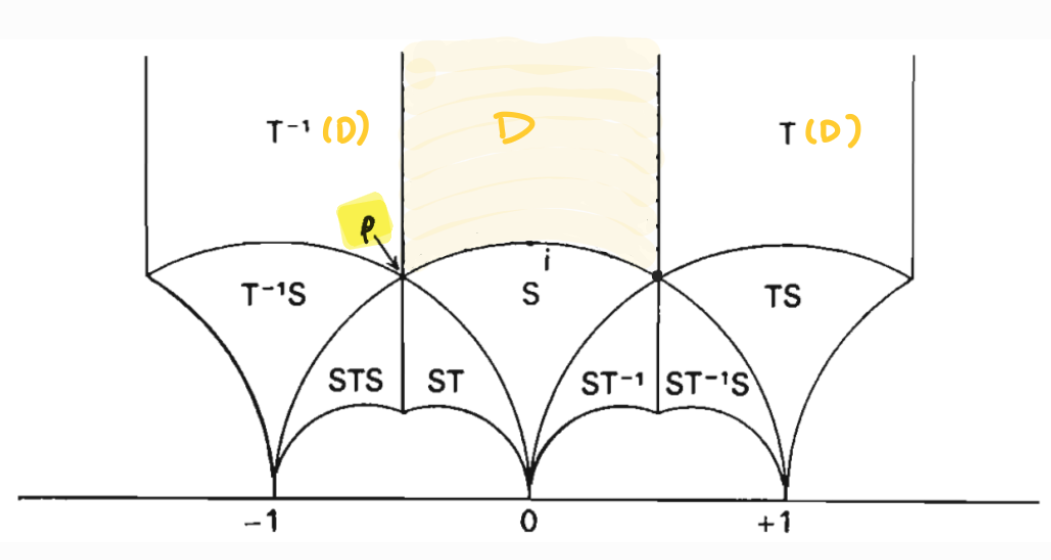
\includegraphics[width=0.7\textwidth]{Fig3.png}
        \caption{}
    \end{figure}
    \begin{thm}[label=thm2]
    \begin{enumerate}[(i)]
        \item For every \(z\in \mathbb{H} \), there exists \(g \in G\) such that \(gz\in D\).
        \item Suppose that two distinct points \(z,z^{\prime} \)  of \(D\) are congruent modulo \(G\). Then, \(\Re(z) = \pm 1/2\) and \(z=z^{\prime} \pm 1\), or \(\vert z \vert =1\) and \(z^{\prime} =-1/z\) 
        \item Let \(z\in D\) and let \(I(z)=\left\{g \mid g\in G, gz=z \right\}\) the stabilizer of \(z\) in \(G\). One has \(I(z)=\{1\}\) except in the following cases:
        \begin{enumerate}[label=(\alph*)]
            \item \(z=i\) in which case \(I(z)\) is the group of order \(2\) generated by S;
            \item \(z=\rho = e^{2\pi i/3}\), in which case \(I(z)\) is the group of order \(3\) generated by \(ST\) ;
            \item \(z=-\hat{\rho} = e^{\pi i/3}\), in which case \(I(z)\) is the group of order \(3\) generated by \(TS\)
        \end{enumerate}
    \end{enumerate}
    \end{thm}
    
    \begin{proof}~\\
        (i) Let \(G^{\prime} \subset G  \) be the subgroup generated by \(S\) and \(T\) and let \(z\in \mathbb{H} \). We seek to prove that there exsits \(g^{\prime} \in G^{\prime} \) such that \( g^{\prime} z\in D\) which will prove assertion (1). If \(g = \begin{pmatrix}
            a &  b \\
            c &  d \\
        \end{pmatrix}\) is an element of \(G^{\prime} \) then as before \(\Im(gz)=\frac{\Im(z)}{\vert cz+d \vert^{2} }\). Since \(c\) and \(d\) are integers, the number of pairs \((c,d)\) such that \(\vert cz+d \vert \) is less than a given constant is finite, thus there is a choice \( g\in G^{\prime} \) such that \(\Im(gz)\) is maximized.\\
        Chose \(n\in \Z\) such that \(-1/2 < \vert < \Re (T^{n}gz)  \vert 1/2\) (show that this necessarily exists). The element \(z^{\prime} =T^{n}gz \) belongs to \(D\) as \(\vert z \vert \geq 1\) because otherwise the element \(\Im(-1/z^{\prime} )> \Im(z^{\prime} )\) which is impossible. Set \( g^{\prime} =T^n g\) which is the element we are looking for and note that
        \(T^n = \begin{pmatrix}
            1 &  n \\
            0 &  1 \\
        \end{pmatrix} \)  \qed\\
        Now let \(z\in D\) and \( g = \begin{pmatrix}
            a &  b \\
            c &  d \\
        \end{pmatrix}\in G\) such that \(gz\in D\). We may assume \(\Im(gz)\geq \Im(z)\) i.e \(\vert cz+d \vert^2 \leq 1\) by replacing the pair \((z,g)\) by \((gz,g^{-1} )\) if needed. Since \(c\) is an integer, the only cases to check which satisfy this inequality are \(c=-1,0,1\).\\[12pt]
        If \(c=0\) then \(d=\pm 1\) for which \(g = \begin{pmatrix}
            1 &  \pm b \\
            0 & 1  \\
        \end{pmatrix}\) so that \(g\) acts by translation, i.e \(gz = z \pm b\). Since both \(\vert \Re (z) \vert, \vert \Re (gz) \vert <1/2\) then either \( b=0, g = 1\) or \( b= \pm 1\) in which case  \(\Re (z) = \pm 1/2\) and \(\Re (gz) = -\Re (z)\).\\[6pt]
        If \(c=1\) then \(\vert cz+d \vert \leq 1\) implies \(\vert z+d \vert \leq 1\). Hence \(d=0\) except when \(z=\rho,\widetilde{-\rho } \), in which cases \(d=0,1\) or \(d=0,-1\)
        If \(d=0\), \(\vert z \vert \leq 1\) so \(\vert z \vert =1\) since we are in \(D\). But \(ad-bc=1\) implies \(b=-1\). Hence \(gz=a-1/z \in D\)so as above, \(a=0\) or \(\Re(-1/z)=\pm 1/2\). Then \(-1/z\in D\), \(\vert -1/z \vert =1\) thus \(-1/z=\rho \) or \(-\widetilde{\rho } \) and \(z=\rho \) or \(-\widetilde{\rho } \). In these cases, \(a=0,-1\) for \(z=\rho \) and \(a=0,1\) for \(z\setminus \widetilde{\rho } \).\\[6pt]
        If \(d=1\), \(z=\rho \) gives \(a=b=1\) so \(g \rho =\frac{a-1}{1+\rho } = a+\rho \) thus \(a=0,1\)\\[6pt]
        If \(d=-1, z=-\widetilde{\rho } \) then \( g (-\widetilde{\rho } ) = (a+(-\widetilde{\rho } ) )  \) similarly and \(a=0,-1\).
        This proves (ii). \qedhere
        
        For (iii), suppose \(g\in G\), \(z\in D\) and \(gz=z\). In particular, \(gz\in D\) so we can use what we did for \((ii)\). There are two possibilities:\\[6pt]
        If \(c=0\), then \(g\) is given by \(\begin{pmatrix}
            \pm 1 &  b   \\
             0 & \pm 1  \\
        \end{pmatrix} \) but \(gz=z\) means \(b=0\) so \(g=1_G\).\\[6pt]
        
        If \(c= \pm 1\), then there are three further situations: when \(d=0\), \(g\) is given by \(\begin{pmatrix}
            a &  -1 \\
            1 &  0 \\
        \end{pmatrix}\). We know \(gz\in D\) if and only if \(a=0\) and \(\vert z \vert =1\) or \(z=\rho \) and \(a=0,-1\) or \(z=-\widetilde{\rho } \) and \(a=0,1\). But out of these possibilities we only have \(gz=z\)  \(z=i \mapsto a=0\) or \(z=\rho \mapsto a=-1\) or \(z=-\widetilde{\rho }\mapsto a=-1 \). \\[6pt]
        When \(d=1\), then \(z=\rho \) and \(a=0\) (to have \(gz=z\) ).\\[6pt]
        When \(d=-1\) then \(z=-\widetilde{\rho } \) and \(a=0\).                    
    \end{proof}
    
    Then assertions (1) and (2) imply 
    \begin{cor}
    The canonical map \(D\to \mathbb{H} /G\) is surjective and its restriction to the interior of \(D\) is injective.
    \end{cor}
    \begin{thm}[label = gen]
    The group \(G\) is generated by \(S\) and \(T\).
    \end{thm}
    \begin{proof}
    Let \(G^{\prime} \) be the subgroup generated by \(S,T\) once more and \(g\in G\). 

    Choose a point \(z_0 \in \mathring{D}\) and let \(z=gz_0\). Since by \cref{thm:thm2}, there exists \(g^{\prime} \in G^{\prime} \) such that \(g^{\prime} z \in D\), the points \(z_0\) and \(g^{\prime} z=g^{\prime} gz_0\) of \(D\) are congruent modulo \(G\) and one of them is in \(\mathring{D}\). 
    
    By assertions (2) and (3), the two points coincide and \(g^{\prime} g=1\), hence \(g\in G^{\prime} \) as desired.
    \end{proof}
\section{Modular Functions}
\subsection{Defintions}
\begin{dfn}[label = wm]
We say a function \(f\) is \textbf{weakly modular of weight} \(2k\) if is meromorphic on the half plane \(\mathbb{H}\) and verifies the relation
\[
    f(z)= (cz+d)^{-2k}f\left(\frac{az+b}{cz+d}\right),\quad \forall \begin{pmatrix}
        a &  b \\
        c &  d \\
    \end{pmatrix} \in \SL, \, k\in\Z
\]
\end{dfn} 
We denote \(g\) as the image of $\begin{pmatrix}
    a &  b \\
    c &  d \\
\end{pmatrix}$ in \(G\). Then
\[
    \frac{\mathrm{d}(gz)}{\mathrm{d}z} = \frac{\mathrm{d}}{\mathrm{d}z} \left(\frac{az+b}{cz+d}\right) = \frac{(cz+d)(a)-(az+b)(c)}{(cz+d)^2} = \frac{ad-bc}{(cz+d)^2} = \frac{1}{(cz+d)^2}
\] 
Then by \cref{dfn:wm} 
\[
    f(z) = (cz+d)^{-2k} f(gz) \implies \frac{f(gz)}{f(z)} = \left(\frac{\mathrm{d}(gz)}{\mathrm{d}z} \right)^{-k} \iff f(gz)\mathrm{d}(gz)^k = f(z)\mathrm{d}z^k  
\]
This is to be read as the \textit{differential form of weight} \(k\), \(f(z)\mathrm{d}z^k \) is invariant under \(G\).

\cref{thm:gen} shows \(G\) is generated by \(S\) and \(T\), so  we only need to check the invariance on these generators.
\begin{prop}
Let \(f\) be meromorphic on \(\mathbb{H}\). The function \(f\) is a weakly modular function of weight \(2k\) if and only if it satisfies the two relations:
\begin{align*}
f(z+1) = f(z) \quad (f(Tz)=f(z))\\
f\left(\frac{-1}{z}\right) = z^{2k}f(z) \quad (f(Sz) = z^{2k}f(z))
\end{align*}
\end{prop}  
\begin{proof}
\(\implies\)

\smallskip 
Suppose \(f\) is weakly modular, then taking \(g = T \in \SL\), we see
\[
    f(z) = 1^{-2k} f\left(\frac{z+1}{1}\right) = f(z+1)
\] 
and taking \(g= S\) instead
\[
    f(z) = z^{-2k} f\left(\frac{-1}{z}\right) \implies f\left(\frac{-1}{z}\right) = z^{2k}f(z)
\] 
\(\impliedby\)

\smallskip
Suppose the two relations are satisfied, then since \(S\) and \(T\) generate \(G\), for any \(g\in G\), we can find \(f(gz)\) by applying the respective relations implied by \(S\) and \(T\). We need only show that the correct factor of \((cz+d)^{-2k}\) arises. 
Let 
\[
    T = \begin{pmatrix}
        1 &  1 \\
        0 &  1 \\
    \end{pmatrix}, \quad S = \begin{pmatrix}
        0 &  -1 \\
        1 &  0 \\
    \end{pmatrix}, \quad V = \begin{pmatrix}
        a & b  \\
        c & d  \\
    \end{pmatrix} \in \SL
\] 
Note that since \(S^2 = -1 \equiv 1 \Mod{G}\), then start with base cases \(V=T\) and \(V=S\) and using induction on  
\[
    V = T^{n_1}S T^{n_2}S T^{n_3}S\dots
\] 
it becomes trivial to see the correct factor fall out.
\end{proof}

By the first relation, we can show that \(f\) may be expressed as a function of \(q=e^{2 \pi i z}\). 
\begin{proof}
Indeed, since \(f(z)=f(z+1)\), then \(f\) is \(1\)-periodic. We can then define an equivalence relation on \(\mathbb{H}\) by
\[
    z \sim w \iff z - w \in \mathbb{Z}.
\]     
So that the new domain of interest is the image of \(\mathbb{H}\) in \(\quot{\mathbb{C} }{\mathbb{Z} } \). Let 
\begin{align*}
q: \quot{\mathbb{C} }{\mathbb{Z} } &\to \mathbb{C} \\
z &\mapsto e^{2\pi iz} 
\end{align*}
This map is well-defined because if \([z]=[z^{\prime} ]\) (i.e. \(z = z^{\prime} +k\) for some \(k \in \mathbb{Z} \)) then
\[
    q(z) = e^{2\pi  i z} = e^{2\pi i z}e^{2\pi i k} = e^{2\pi i(z+k)} = q(z^{\prime} )
\] 
and furthermore this map is injective because
\[
    e^{2 \pi i z} = e^{2\pi i w} \iff e^{2\pi i (z - w)} = 1 \iff z - w \in \Bbb{Z} \iff z \sim w.
\]
which implies that \(q\) has a left inverse, \(p: \mathbb{C} \to \quot{\mathbb{C} }{\mathbb{Z} } \) so that \(p\circ q = \Id_{ \mathbb{C} / \mathbb{Z} } \). 

\(f\), being \(1\)-periodic, can be considered as a function from \(\quot{\mathbb{C} }{\mathbb{Z} } \to \mathbb{C} \), whence
\[
    f = f \circ \Id_{\mathbb{C} /\mathbb{Z} } = f \circ (p \circ q) = (f \circ p) \circ q \colon \quot{\mathbb{C} }{\mathbb{Z} } \to  C 
\]
So we see that \(f\) can be written as a function of \(q\) and hence denote \[\widetilde{f}(q(z)) = (f \circ p)(q(z)), z\in \mathbb{C}  \]  
and essentially \(\widetilde{f}(z) = f \left(\frac{\log q}{2\pi i}\right) = \widetilde{f} (q)\) 
\end{proof}  
Since \(f\) is meromorphic on \(\mathbb{H}\), then \(\widetilde{f} \) is meromorphic on \(D\coloneqq \{ q(z) \mid |q|<1, q(z) \ne 0\} \)

If \(\widetilde{f} \) extends to a meromorphic (resp. holomorphic) function at the origin, we say, BY ABUSE OF LANGUAGE, that \(f\) is meromorphic (resp. holomorphic) at infinity, i.e. \(\widetilde{f} \) admits a Laurent expansion around a neighborhood of \(0\)
\[
    \widetilde{f}(q) = \sum_{-\infty }^{\infty} a_{n}q^n   
\]    where \(a_n = 0 \) for \(n \) small enough (resp. for \(n<0\) ).

\begin{dfn}
A weakly modular function is called \textbf{modular} if it is meromorphic at infinity. We set \(f(i\infty )= \widetilde{f}(0) \) and call it the \textbf{value at infinity}  
\end{dfn}
\begin{dfn}
A modular function which is holomorphic everywhere (including infinity) is called a \textbf{modular form}; if such a function is zero at infinity, it is called a \textbf{cusp form} ("Spitzenform" in German --- "forme parabolique" in French)  
\end{dfn}
Then a modular form of weight \(2k\) admits power series expansions
\[
    f(z) = \sum_{0}^{\infty} a_n q^n = \sum_{0}^{\infty} a_n e^{2\pi i n z}
\]
which converges when \(\vert q \vert <1\) (i.e. for \(\Im (z)>0\) ) which is obviously \(1\)-periodic and VERIFY
\[
    f\left(\frac{-1}{z}\right) = z^{2n}f(z)
\]
and is a cusp form when \[f(i \infty ) = 0 \implies \widetilde{f} = 0 \implies a_{0}=0 \]

\begin{claim}
    If \(f\) and \(f^{\prime} \) are of weight \(2k\) and \(2k^{\prime} \), respectively, the product \(f f^{\prime} \) is a modular form of weight \(2k+2k^{\prime} \)     
\end{claim}
\begin{proof}
    Obviously as
    \[
        f(z)f^{\prime}(z) = (cz+d)^{-2k} f(gz) (cz+d)^{-2m} f^{\prime} (gz) = (cz+d)^{-2(k+m)} (f\cdot f^{\prime} )(gz)
    \]
\end{proof}

\subsection{Lattice functions and modular functions}

\begin{dfn}
Let \(V\) be a real vector space of finite dimension. Then a subgroup \(\Gamma \) is called a \textbf{lattice} if it satisfies one of the following equivalent conditions:
\begin{enumerate}[label=(\alph*)]
    \item \(\Gamma \) is discrete and \(V/\Gamma \) is compact;
    \item \(\Gamma \) is discrete and generates the \(\mathbb{R} \)-vector space \(V\);
    \item There exists an \(\mathbb{R} \)-basis \((e_1,\dots,e_n)\) of \(V\) which is a \(\mathbb{Z} \)-basis of \(\Gamma \) (i.e. \(\Gamma = \mathbb{Z} e_1 \oplus  \dots \oplus \mathbb{Z} e_n\))        
\end{enumerate}   
\end{dfn}

Denote the set of lattices of \(\mathbb{Z} \)  by \(\mathscr{R} \) (here \(\mathbb{C} \) is considered as a dimension two real vector space ). Let \(M\) be the set of pairs \((\omega_1, \omega _2) \in \mathbb{C} ^{\ast} \times \mathbb{C} ^{\ast} \) such that \(\Im(\omega _1/\omega _2)>0\),i.e
\[
    M \coloneqq \{ (\omega _1,\omega _2)\in \mathbb{C} ^{\ast} \times \mathbb{C} ^{\ast} : \Im (\omega_1/\omega _2)>0 \} 
\] To such a pair we associate the lattice
\[
    \Gamma (\omega _1,\omega _2) = \mathbb{Z} \omega _1 \oplus \mathbb{Z} \omega _2
\]  
with basis given by \((\omega_1,\omega _2)\). 

\begin{claim}
    The map \(\Gamma : M \to \mathscr{R} \) is surjective 
\end{claim}
\begin{proof}
    Indeed, if \(\Gamma \) is a lattice (using definition (c)) then there exist \(\omega _1,\omega _2\), a basis of \(\mathbb{C} \) (a basis of \(\mathbb{R} ^2\)), such that \[\Gamma = \mathbb{Z} \omega _1\oplus \mathbb{Z} \omega _2\] Since they form a basis, neither are \(0\) so that \((\omega_1,\omega _2) \in\mathbb{C} ^{\ast} \times \mathbb{C} ^{\ast}  \). That is, \((\omega _1,\omega _2)\) generate \(\Gamma \) as a \(\mathbb{Z} \)-module       

    Either \(\omega_1/\omega _2\) already lies in the upper half-plane or if it doesn't, we can reorder the basis and then \(\omega_2/\omega_1\) will.   
\end{proof}

Let \(g = \begin{pmatrix}
    a &  b \\
    c &  d \\
\end{pmatrix} \in \SL\) and let \((\omega _1,\omega _2) \in M\). Set \( \omega_1^{\prime} \coloneqq a \omega _1 + b \omega _2,\omega_2^{\prime} \coloneqq c \omega _1 + d\omega _2 \) so that
\[
    g \cdot (\omega _1,\omega _2) \coloneqq \begin{pmatrix}
        a &  b \\
        c &  d \\
    \end{pmatrix}\begin{pmatrix}
         \omega_1 \\ \omega_2
    \end{pmatrix} = (a \omega _1 + b \omega _2 , c \omega _1 + d\omega _2) = (\omega_1^{\prime} ,\omega _2^{\prime} )
\]  
Then we see that 
\begin{align*}
    \Gamma (\omega _1^{\prime} ,\omega _2^{\prime} ) = \mathbb{Z} \omega _1^{\prime}  \oplus \mathbb{Z} \omega _2^{\prime}  = \mathbb{Z} (a \omega_1 + b \omega _2)  \oplus \mathbb{Z} (c \omega_1 + d \omega _2) 
\end{align*}
so that \(\{ \omega _1^{\prime} ,\omega _2^{\prime}  \} \) is also a basis of \(\Gamma (\omega _1, \omega _2)\). Then set \(z = \omega_1/\omega _2\) and \(z^{\prime} = \omega _1^{\prime} / \omega _2^{\prime} \) and hence
\[
    z^{\prime} = \frac{ a \omega _1 + b \omega _2 }{c \omega _1 + d\omega _2 } = \frac{a \left(\frac{\omega _1}{\omega _2}\right) + b }{ c \left(\frac{\omega _1}{\omega _2}\right) + d} = \frac{az+b}{cz+d} = gz
\]    
which shows \(\Im(z^{\prime} )>0\) (since \(\mathbb{H} \) is stable under the action of \(\SL\) and thus \((\omega _1^{\prime} ,\omega _2^{\prime} )\in M\) 

\begin{prop}[label=cong]
For two elements of \(M\) to define the same lattice, it is necessary and sufficient that they are congruent modulo \(\SL\) 
\end{prop}
\begin{proof}
Above we have shown one direction, where if  they are congruent modulo \(\SL \), i.e 
\[
    \begin{pmatrix}
         \omega _1^{\prime} \\ \omega _2^{\prime} \\
    \end{pmatrix} = \begin{pmatrix}
        a &  b \\
        c &  d \\
    \end{pmatrix} \begin{pmatrix}
        \omega _1  \\
        \omega _2  \\
    \end{pmatrix} \quad \begin{pmatrix}
        a &  b \\
        c &  d \\
    \end{pmatrix}\in\SL
\]  
then they define the same lattice. 

In the other direction, suppose \((\omega _1,\omega _2)\) and \(\omega _1^{\prime} ,\omega _2^{\prime} \) define the same lattice. Then there are integers \(a,b,c,d,e,f,g,h \in \mathbb{Z} \) such that 
\[
    \begin{pmatrix}
        a &  b \\
        c &  d \\
    \end{pmatrix} \begin{pmatrix}
        \omega _1  \\
        \omega _2  \\
    \end{pmatrix} = \begin{pmatrix}
        \omega _1^{\prime}   \\
        \omega _2^{\prime}   \\
    \end{pmatrix} \quad \begin{pmatrix}
        e&  f \\
        g &  h \\
    \end{pmatrix} \begin{pmatrix}
        \omega _1^{\prime}   \\
        \omega _2 ^{\prime}  \\
    \end{pmatrix} = \begin{pmatrix}
        \omega _1  \\
        \omega _2  \\
    \end{pmatrix}
\]  
but then this implies
\[
    \begin{pmatrix}
        a &  b \\
        c &  d \\
    \end{pmatrix}\begin{pmatrix}
        e&  f \\
        g &  h \\
    \end{pmatrix} = \begin{pmatrix}
        1 &  0 \\
        0 &  1 \\
    \end{pmatrix}
\]
Then, since the entries are integers, taking determinants on both sides we see that the determinant of each matrix is \(\pm 1\). But since \(\Im (\omega_1/\omega _2)>0\) and \(\Im (\omega_1^{\prime} /\omega _2^{\prime} )>0\), the determinants can not be negative otherwise these ratios would have opposite imaginary parts. Therefore, they differ exactly by matrices in \(\SL\).    
\end{proof}
Therefore, we have a bijection
\[
    \mathscr{R} \longleftrightarrow \quot{M}{\SL} 
\] 
Now let \(\mathbb{C} ^{\ast} \) act on \(\mathscr{R} \) (resp. on M) By 
\[
    \Gamma \mapsto \lambda \Gamma \quad (\textrm{resp. } (\omega _1,\omega _2) \mapsto (\lambda \omega _1,\lambda \omega _2)), \quad \lambda \in \mathbb{C} ^{\ast} 
\]  
\begin{prop}
The map \((\omega _1,\omega _2)\mapsto \omega _1/\omega _2\) gives, by passing to the quotient, a bijection of \(\quot{\mathscr{R} }{\mathbb{C} ^{\ast} } \) onto \(\quot{\mathbb{H}}{G} \). Thus, an element of \(\quot{\mathbb{H}}{G} \) can be identified with a lattice of \(\mathbb{C} \) defined up to homothety (i.e. \(\Gamma ^{\prime} = \lambda \Gamma \) for some \(\lambda \in \mathbb{C} ^{\ast} \)  )    
\end{prop}
\begin{proof}
By the action of \(\mathbb{C} ^{\ast} \) on \(\mathscr{R} \), we have the well defined bijection
\begin{align*}
\Psi: \quot{M}{\mathbb{C} ^{\ast} } &\longleftrightarrow \mathbb{H} \\
(\omega_1,\omega_2) &\mapsto \omega_1/\omega_2\\
(z,1) &\mapsfrom z 
\end{align*}   
Now let \(g\in \SL\), then we have
\begin{align*}
\Psi(g\cdot (\omega _1,\omega _2)) = g \cdot \Psi (\omega_1,\omega_2)\\
\frac{a \omega _1 + b \omega _2}{c \omega _1 + d \omega _2}  = \frac{a \left(\frac{\omega_1}{\omega_2}\right) +b }{c \left(\frac{\omega_1}{\omega_2}\right) +d}
\end{align*} 
Thus
\[
    \frac{\quot{M}{\mathbb{C}^{\ast} } }{\SL} \underset{\textrm{nat bij}}{\Longleftrightarrow} \quot{\mathbb{H} }{G} 
\]
But
\begin{align*}
    \frac{\quot{M}{\mathbb{C}^{\ast} } }{\SL} &\cong \frac{\mathscr{R} }{\mathbb{C} ^{\ast} }\\
    \lambda (\omega _1,\omega _2)&\mapsto \lambda \Gamma (\omega _1,\omega _2)
\end{align*}
\end{proof}

\begin{remark}
    Every lattice \(\Gamma \) can be associated to the elliptic curve \(\quot{\mathbb{C} }{\Gamma } \). Then two lattices define isomorphic elliptic curves if and only if they are homothetic. Thus the bijection in the previous proposition can be thought of as isomorphism classes of elliptic curves.
\end{remark}

Let \(F:\mathscr{R} \to \mathbb{C} \) and \(k\in \mathbb{Z} \). We say that \(F\) is of \textit{weight} \(2k\) if for all \(\Gamma \in \mathscr{R} \) and \(\lambda \in \mathbb{C} ^{\ast} \), the following holds 
\[
    F(\lambda \Gamma ) = \lambda ^{-2k}F(\Lambda )
\]   
If \((\omega _1,\omega _2)\in M\), then denote \(F(\omega _1,\omega _2)\) to be the value \(F(\Gamma (\omega _1,\omega _2))\). Then the previous relation becomes
\[
    F(\lambda \omega _1,\lambda \omega _2) = \lambda ^{-2k} F(\omega _1,\omega _2)
\]   
\begin{claim}
    \(F(\omega _1,\omega _2)\) is invariant by the action of \(\SL\) on \(M\)   
\end{claim}
\begin{proof}
\cref{prop:cong} shows that the action of \(\SL\) preserves the lattice structure, hence the image of a lattice \(\Gamma \) under \(F\) is also preserved by this action
\[
    F(\Gamma ) = F(g \Gamma ),\quad g \in \SL
\]
\end{proof}
\begin{claim}
    The product \(\omega_2^{2k}F(\omega _1,\omega _2)\) only depends on \(z=\omega _1/\omega _2\)  
\end{claim}
\begin{proof}
Suppose \(\omega_1/\omega_2 =\omega_1^{\prime} /\omega_2^{\prime}  \). Then
\begin{align*}
    \omega_2^{2k}F(\omega _1,\omega _2) = \omega_2^{2k}F\left(\omega _2 \left(\frac{\omega_1 }{\omega_2}\right),\omega _2\left(\frac{\omega_2 }{\omega_2}\right)\right) = F(\omega_1/\omega_2,1) \\= F(\omega_1^{\prime} /\omega_2^{\prime} ,1) \\= (\omega_2^{\prime})^{2k}F(\omega _1^{\prime} ,\omega _2^{\prime} ) 
\end{align*}
So, \(\omega_2^{2k}F(\omega _1,\omega _2)\) is a function of \(\omega_1/\omega_2\), an element of \(\mathbb{H} \).   
\end{proof}
Thus, as a result, there exists a function \(f:\mathbb{H}\to  \mathbb{C} \) such that
\[
    F(\omega _1,\omega _2) = \omega _2^{-2k} f(\omega _1/\omega _2)
\] 
Since \(F\) is invariant by \(\SL\), we see that \(f\) satisfies 
\begin{align*}
    \omega _2^{-2k} f(\omega _1/\omega _2) = (c \omega _1 + d \omega _2)^{-2k} f\left(\frac{a \omega _1 + b \omega _2}{ c \omega _1 + d \omega _2}\right) 
\end{align*}

Let \(z\in \mathbb{H} \) and take \((\omega _1,\omega _2) = (z,1)\), then \(f\) satisfies the modular relation 
\[
    f(z) = (cz+d)^{-2k} f\left(\frac{az+b}{cz+d}\right), \quad \forall z \in \mathbb{H} 
\] 
It also holds that we can associate any function \(f\) which satisfies this relation to a function \(F:\mathscr{R} \to  \mathbb{C} \) of weight \(2k\). Indeed, define 
\begin{align*}
F: M &\to  \mathbb{C} \\
(\omega_1,\omega _2) &\mapsto \omega _2^{-2k}f(\omega_1/\omega_2)
\end{align*}
Then this satisfies the invariance under \(\SL\) and the relation \(F(\lambda \omega _1,\lambda \omega _2) = \lambda ^{-2k} F(\omega _1,\omega _2)\). So let 
\begin{align*}
F: \mathscr{R} &\to \mathbb{C} \\
\Gamma_0 &\mapsto F(\Gamma_0 )\coloneqq F((\omega _1,\omega _2))
\end{align*}
with \((\omega _1,\omega _2)\) any element in \(M\) such that \(\Gamma ((\omega _1,\omega _2))=\Gamma _0\)   
With these realizations, we have proved the correspondence
\[
    \{ \textrm{modular functions of weight } 2k \longleftrightarrow \textrm{lattice functions of weight } 2k \} 
\]   

\subsection{Examples of modular functions; Eisenstein series}
\begin{lem}
Let \(\Gamma \) be a lattice in \(\mathbb{C} \). The series
\[
    \sum_{\gamma \in \Gamma\setminus \{ 0 \}  }\frac{1}{\vert \gamma \vert^\sigma  } 
\]  
converges for \(\sigma >2\) 
\end{lem}
\begin{proof}
Let \(\delta \) be the minimum distance between points in \(\Gamma \) and consider the annulus 
\[
    A \coloneqq \{ z\in \mathbb{C} \mid r< \vert z \vert <r+\delta /2 \} 
\]   
Any two lattice points in this annulus are separated by an arc along the inner radius of length at least \(\delta /2\). Then it follows that \(A\) contains at most \(4\pi r/\delta \) lattice points and the number of lattice points in an annulus \(\{n\leq \vert \gamma\vert \leq n+1\}\) is bounded above by \(cn\), where 
\[
    c \leq \frac{2}{\delta } \cdot \frac{4\pi r}{\delta } = \frac{8\pi }{\delta ^2}
\]      
Then we have 
\[
    \sum_{\substack{\gamma \in \Gamma\setminus \{ 0 \} \\ \vert \gamma  \vert \geq 1  }} \frac{1}{\vert \gamma  \vert^\sigma  }\leq  \sum_{n=1}^{\infty} \frac{cn}{n^k} = c \sum_{n=1}^{\infty} \frac{1}{n^{k-1}}<\infty   
\]
since \(\sigma >2\). Thus we see 
\[
    \sum_{\gamma \in \Gamma\setminus \{ 0 \}  } \frac{1}{\vert \gamma  \vert^\sigma  } = \sum_{\substack{\gamma \in \Gamma\setminus \{ 0 \}\\0< \vert \gamma  \vert <1} } \frac{1}{\vert \gamma  \vert^\sigma  } + \sum_{\substack{\gamma \in \Gamma\setminus \{ 0 \}\\ \vert \gamma  \vert \geq 1  }} \frac{1}{\vert \gamma  \vert^\sigma  } <\infty 
\] 
since the first summation is also clearly bounded.
\end{proof}

\begin{dfn}
For \(k>1\) and \(\Gamma \in \mathscr{R} \), the \textbf{Eisenstein series of index} \(k\) is defined as
\[
    G_k(\Gamma )\coloneqq \sum_{\gamma \in \Gamma\setminus \{ 0 \}  } \frac{1}{\gamma ^{2k}} 
\]    
which converges absolutely by the previous lemma
\end{dfn}
By the bijection in the previous section, we can also view \(G_k\) as
\[
    G_k(\omega _1,\omega _2) = \sum_{(m,n)\in (\mathbb{Z} \times \mathbb{Z}) \setminus \{ 0 \}  }\frac{1}{(m \omega _1+ n \omega _2)^{2k}}
\] 
Then, this is a lattice function, and from the previous discussion we know
\begin{align*}
    &G_k(\omega _1,\omega _2) = \sum_{(m,n)\in (\mathbb{Z} \times \mathbb{Z}) \setminus \{ 0 \}  }\frac{1}{(m \omega _1+ n \omega _2)^{2k}} = \omega _2^{-2k} f(\omega_1/\omega_2)\\  &\implies G_k(z) = \sum_{(m,n)\in (\mathbb{Z} \times \mathbb{Z}) \setminus \{ 0 \}  }\frac{1}{(m z+n)^{2k}}
\end{align*}
which is also absolutely convergent and \(z=\omega_1/\omega _2\) . The function on \(\mathbb{H}\) corresponding to \(G_k\) is, by slight abuse of notation, also denoted \(G_k\) (this is okay because of the procedure from the previous section). 
\begin{prop}[label=eisen]
Let \(k>1\) be an integer. The Eisenstein series \(G_k(z)\) is a modular form of weight \(2k\). We have \(G_k(i\infty ) = 2\zeta (2k)\) where \(\zeta \) denotes the Riemann zeta function. Actually, one can show
\[
    G_k(z) = 2 \zeta (2k) + \frac{2^{k+1}\pi ^{2k}(-1)^k}{(2k-1)!} \sum_1^{\infty} \sigma_{2k-1}(n)e^{2\pi inz}
\]
where \(\sigma_k(n) = \sum_{d \mid n} d^k\). 
\end{prop}
\begin{proof}
We have already shown \(G_k(z)\) is a weakly modular function of weight \(2k\), that is
\[
    G_k(z) = (cz+d)^{-2k}G_k\left(\frac{az+b}{cz+d}\right), \quad \forall z\in \mathbb{H}, g = \begin{pmatrix}
        a &  b \\
        c &  d \\
    \end{pmatrix} \in \SL
\] 
It remains to show that it is holomorphic everywhere (including infinity).

Recall a theorem of Weierstrass in complex analysis
\begin{thm}
Suppose \(\{ f_n \} \) is a sequence of functions holomorphic on an open set \(\Omega \) and that \(\{ f_n \} \) converges to a function \(f\) uniformly on every compact subset of \(\Omega \). Then \(f\) is holomorphic on \(\Omega \).      
\end{thm}
We have that the truncated series defined by \(G_k(z)\) is uniformly and absolutely convergent and each term of the series is holomorphic on \(\mathbb{H} \), so necessarily by the theorem \(G_k(z)\) is holomorphic on all of \(\mathbb{H} \).

Finally, we check holomorphicity at \(i\infty \). Since we know \(G_k(z)\) is weakly modular, we need only look at its behavior on the fundamental domain \(D\). In view of the uniform convergence in \(D\), we check \(G_k(i\infty )\) in a term by term limit. For \(z\ne 0\), we have  
\[
    \lim_{\Im z \to \infty }G_k(z) = \sum_{\substack{m,n\in \mathbb{Z}\\(m,n)\ne (0,0)}} \left(\lim_{\Im z \to \infty } \frac{1}{(mz+n)^{2k} }\right) 
\]    
When \(m \ne 0\), the summation vanishes. So assume \(m = 0\), then it becomes
\[
    \sum_{n\ne 0} \frac{1}{n^{2k} } = 2 \sum_{n=1}^{\infty} \frac{1}{n^{2k} } = 2 \zeta (2k)  
\] 
\end{proof}

The Eisenstein series of lowest weights are when \(k=2,3\) which make \(G_2\) and \(G_3\) modular forms of weight \(4\) and \(6\) respectively. The theory of elliptic curves suggests the convenience of defining the multiples
\[
    g_2=60G_2, \quad g_3 =140G_3
\]
Then we have
\begin{align*}
g_2(i\infty ) = 120\zeta(4) = \frac{4}{3}\pi ^4, \quad g_3(i\infty ) = \frac{8}{27}\pi ^6
\end{align*} 
Then set \(\Delta =g_2^3 - 27g_3^2\).
\begin{claim}
    \(\Delta \) is a cusp form of weight \(12\).  
\end{claim}
\begin{proof}
Clearly \(g_2^3\) is a modular form of weight \(4\cdot 3=12\) and \(g_3^2\) is a modular form of weight \(6\cdot 2=12\), therefore \(\Delta \) is one as well. We need only check the value of \(\Delta \) at \(i\infty \).
\[
    \Delta (i\infty ) =g_2^3(i\infty ) - 27 g_3^2(i\infty ) = \left( \frac{4}{3} \right)^3 \pi^{12} - 27 \left( \frac{8}{27} \right)^2 \pi ^{12} =0
    \]       
\end{proof}

Recall the Weierstrass function associated to \(\Gamma \)
\[
    \wp_\Gamma (u) = \frac{1}{u^{2} }+\sum_{\gamma \in \Gamma \setminus \{ 0 \} }\left(\frac{1}{(u-\gamma )^2} - \frac{1}{\gamma ^2}\right) 
\] 
In the Laurent expansion of \(\wp_\Gamma\), we see
\[
    \wp_\Gamma (u) = \frac{1}{u^{2} } + \sum_{k=2}^{\infty} (2k-1)G_k(\Gamma )u^{2k-2} 
\] 
and setting \(x = \wp_\Gamma (u), y = \wp_\Gamma ^{\prime} (u)\), we have
\[
    y^2=4x^3- g_{2} x -g_3 
\] 
Up to a constant, \(\Delta \) as defined above is the discriminant of the polynomial expression on the RHS. One can show that the cubic equation in \(\mathbb{C} \mathbb{P} ^2\) is isomorphic to the elliptic curve \(\mathbb{C} /\Gamma \).
\section{The space of modular forms}
\subsection{The zeros and poles of a modular function}
\begin{dfn}
If \(f \not\equiv 0\) is meromorphic function on \(\mathbb{H}\)  and \(p \in \mathbb{H}\), the integer \(n\) such that \(\frac{f}{(z-p)^n}\) is holomorphic and non-zero at \(p\), denoted by \(v_p(f)\), is called the \textbf{order} or \textbf{valency} of \(f\) at \(p\)
\end{dfn}
\begin{claim}
    \(v_p(f(z))=v_{g(p)}(f(z))\) 
\end{claim}
\begin{proof}
The goal is to use the argument principle around small balls around \(p\) and \(g(p)\). Starting with the modular relation
\[
    f(z) = (cz+d)^{-2k} f(g(z)), \quad \forall g \in \SL
\]
Let \(h(z) = (cz+d)^{2k}\) and note it is holomorphic everywhere on \(\mathbb{H} \). Then taking derivatives we get
\[
    f^{\prime} (z) = h(z) f^{\prime} (gz) g^{\prime} (z) + h^{\prime} (z) f(g(z))
\] 
which gives
\begin{align*}
    \frac{\mathrm{d} f}{f} = \frac{f^{\prime} (z)\mathrm{d} z}{f(z)}&= \frac{h(z)f^{\prime} (g(z)) g^{\prime} (z)+ h^{\prime} (z) f(g(z))}{h(z)f(g(z))}\\
    &= \frac{f^{\prime} (g(z)) g^{\prime} (z) \mathrm{d} z}{f(g(z))} + \frac{h^{\prime} (z)\mathrm{d} z}{h(z)}\\
    &= \frac{\mathrm{d}f(g(z)) }{f(g(z))} + \frac{h^{\prime} (z)\mathrm{d} z}{h(z)}
\end{align*}
By the argument principle and choice of sufficiently small balls \(c_{\epsilon }(p) \) and \(c_{\epsilon }g(p)\), we have
\[
    v_p(f) = \frac{1}{2\pi  i} \int_{c_{\epsilon }(p)} \frac{df(z)}{f(z)}\quad v_p(f) = \frac{1}{2\pi  i} \int_{c_{\epsilon }(g(p))} \frac{df(g(z))}{f(g(z))}
\]
Substituting our derivation, it is immediate
\[
    v_p(f) = \frac{1}{2\pi i} \int_{c_{\epsilon }(p)} \frac{df(z)}{f(z)}= \frac{1}{2\pi i} \int_{c_{\epsilon }(p)} \left(\frac{\mathrm{d}f(g(z)) }{f(g(z))} + \frac{h^{\prime} (z)\mathrm{d} z}{h(z)}\right) = v_{g(p)}f(z) 
\]
since the second integral vanishes as \(h^{\prime} (z)/h(z)\) is holomorphic. 
\end{proof}
Thus, \(v_p(f)\) only depends on the image of \(p\) in \(\quot{\mathbb{H} }{G} \). Furthermore, \(v_{i\infty} (f)\) is defined as the order of \(q=0\) in the extension \(\widetilde{f}(q) \) defined previously.      
Denote the order of the stabilizer of the point \(p\) by \(e_p\). Then 
\[
    e_p = \begin{cases}
        2 & \text{if } p \equiv i \Mod G\\
        3 & \text{if } p \equiv \rho  \Mod G\\
        1 & \text{otherwise}
    \end{cases}
\] 
\begin{thm}[label=val]
Let \(f\) be a modular function of weight \(2k\) not identically zero. One has
\[
    v_{i\infty } (f) + \sum_{p\in \mathbb{H}/G} \frac{1}{e^p}v_p(f) = \frac{k}{6} 
\]
or equivalently
\[
    v_{i\infty }(f) + \frac{1}{2}v_i(f) + \frac{1}{3}v_{\rho }(f) + \sum_{p \in (\mathbb{H}/G)\setminus \{i,\rho   \} } v_p(f)=\frac{k}{6}  
\]
\end{thm}
Since \(\widetilde{f} \) as defined before is meromorphic, there exists \(r>0\) such that \(\widetilde{f} \) has no zeroes or poles in the punctured open disk \(0<\vert q \vert <r\). This is equivalent to saying \(f\) has no zeroes or poles when \(\Im z > \frac{1}{2\pi }\log (1/r)\). Then the portion of the fundamental domain \(D\) defined by the inequality \(\Im z \leq \frac{1}{2\pi }\log (1/r)\) is compact. As \(f\) is meromorphic in \(\mathbb{H}\), it only has a finite number of zeros and poles on this compact set and hence the summation defined above makes sense.
\newpage
\begin{proof}~\\
    \begin{figure}[H]
        \centering
        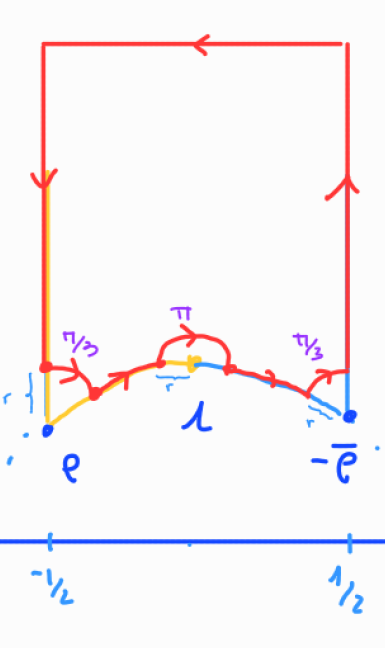
\includegraphics[width=0.35\textwidth]{Fig1.png}
        \caption{The contour \(\mathcal{C}_r\) }
    \end{figure}
Suppose \(f\) has no poles on the boundary of \(D\) except possibly at \(\rho ,-\widetilde{\rho },i \). Then there exists a contour such that its interior contains a representative of each zero or pole of \(f\) not congrunet to \(i\) or \(\rho \). (Note that \(\rho = -1/\widetilde{\rho } \) ), so they are congruent by the \(S\) matrix). \\
Let \(\mathcal{C}_{r} \) denote this contour with the path given by the Figure 1. Then by the argument principle, we know 
\[
    \frac{1}{2\pi i}\int_{\mathcal{C}_{r}} \frac{\mathrm{d} f}{f} = \sum_{p\in (\mathbb{H}/G )\setminus {i,\rho } } v_p(f) 
\]

On the other hand, we can calculate the integral directly along the contour path. There are eight sections of the contour labeled \(C_1,\dots,C_8\) as in the figure.\\[6pt]
For \(C_1\), we have
\begin{align*}
\int_{C_1} \frac{\mathrm{d} f}{f} = \frac{\widetilde{f}(e^{2\pi  iz}) 2 \pi  i z e^{2\pi  iz} }{\widetilde{f}(e^{2\pi iz}) }\mathrm{d} z &= \int_{C_1} \frac{\widetilde{f} ^{\prime} (q(z)) q^{\prime} (z)}{\widetilde{f}(q(z))}\\ &= \int_{q(C_1)} \frac{\widetilde{f}^{\prime} (q) }{\widetilde{f}q }\mathrm{d}q = -2\pi iv_0(\widetilde{f} )\\&=-2\pi iv_{i\infty }(f) \implies \frac{1}{2\pi i}\int_{C_1}\frac{\mathrm{d} f}{f}\mathrm{d}z  =-v_{i\infty }(f)
\end{align*}  
Since \(f(z)=f(z+1)\) we have \(f^{\prime} (z)=f^{\prime} (z+1)\) so clearly
\[
    \int_{C_2}\frac{\mathrm{d} f}{f} = - \int_{C_8} \frac{\mathrm{d} f}{f}
\] 
as \(C_2,C_8\)  have opposite orientation.~\\
If we denote \(C_{p,r,\alpha }\) an arc of a circle of radius \(r\), angle \(\alpha \) centered at \(p\in \mathbb{C} \) with clockwise (negative) orientation, then if \(f\) has a zero or pole at \(p\), we have
\[
    \lim_{r\to 0}\frac{1}{2\pi i}\int_{C_{p,r,\alpha }}\frac{\mathrm{d}f }{f}= -\frac{\alpha }{2\pi } v_p(f) 
\] 
This implies
\begin{align*}
    \lim_{r\to 0}\frac{1}{2\pi i}\int_{C_5}\frac{\mathrm{d}f }{f} = -\frac{1}{2}v_i(f)\\
    \lim_{r\to 0}\frac{1}{2\pi i}\int_{C_3}\frac{\mathrm{d}f }{f} = -\frac{1}{6}v_{\rho } (f)\\
    \lim_{r\to 0}\frac{1}{2\pi i}\int_{C_7}\frac{\mathrm{d}f }{f} = -\frac{1}{6}v_{\widetilde{\rho } }(f) = -\frac{1}{6}v_{\rho }(f)
\end{align*}
Finally, for \(C_4,C_6\), recall that \(Sz=-1/z\) and note that it maps \(C_4\) to \(-C_6\) and also \(f(z) = z^{-2k}f(Sz)\), so that
\[
    f^{\prime} (z)=-2k z^{-2k-1}f(-1/z)+z^{-2k}f^{\prime} (-1/z)(-1/z^2)
\]     

giving
\[
    \int_{C_4}\frac{\mathrm{d}f }{f} = \int_{C_4}\frac{-2k }{z}\mathrm{d}z +\int_{C_4}\frac{f^{\prime} (S(z)) S^{\prime} (z)}{f(S(z))} \mathrm{d}z = \frac{2\pi i k}{6} - \int_{C_6}\frac{f^{\prime} (u) }{f(u)} \mathrm{d} u  
\]
and hence
\[
    \int_{C_4}\frac{\mathrm{d}f }{f}+\int_{C_6}\frac{\mathrm{d}f }{f} = 2\pi i k/6
\]
In total, we collect the equivalent integrations to get
\[
    \sum_{p\in (\mathbb{H}/G )\setminus {i,\rho } } v_p(f) = -v_{i\infty }(f)-\frac{1}{2}v_i(f)-\frac{1}{3}v_{\rho }(f) + \frac{k}{6} 
\]
and rearranging gives the desired relation.\\[6pt]
In the case where \(f\) has zeroes or poles on the half-line
\[
    \{ z \mid \Re(z)=-1/2, \Im z > \sqrt{3}/2  \} 
\]
then \(v_{T \lambda }(f) = v_\lambda (f)\) so we also have the contour in Figure 2
and with a bit more calculation we arrive to the same result.
\begin{figure}[H]
    \centering
    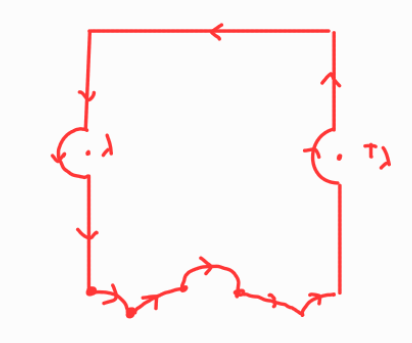
\includegraphics[width=0.35\textwidth]{Fig2.png}
    \caption{}
\end{figure}
Any situation with more poles on the boundary of \(D\) can be dealt similarly.  
\end{proof} 
\subsection{The algebra of modular forms}
If \(k \in \mathbb{Z} \), we denote \(M_k\) the \(\mathbb{C} \)-vector space of modular forms of weight \(2k\) (resp. \(M_k^0\) for cusp forms of weight \(2k\)). By definition of being cusp (\(f(i\infty ) = 0\)), it is clear \(M_k^0\) is the kernel of the linear map 
\begin{align*}
M_k \to \mathbb{C} \\
f \mapsto f(i\infty )
\end{align*}     
Then \(M_k/M_k^0\) has dimension at most \(1\). Moreover, for \(k\geq 2\), the Eisenstein series \(G_k(z)\) is an element of \(M_k\) such that \(G_k(i\infty )\ne 0\) by \cref{prop:eisen}. Hence, we have the isomorphism
\[
    M_k = M_k^0 \oplus \mathbb{C} G_k, \quad k\geq 2
\]    
\begin{thm}[label=33]
    Recalling \(g_2 = 60G_2, g_3 = 140G_3\) and \(\Delta = g_2^3 - 27g_3^2 \in M_6^0\), then
\begin{enumerate}
    \item We have \(M_k=0\) for \(k<0\) and \(k=1\)
    \item For \(k=0,2,3,4,5\), \(M_k\) is a vector space of dimension \(1\) with basis \[\{ 1,G_2,G_3,G_4,G_5 \} \] and \(M_k^0=0\) 
    \item Multiplication by \(\Delta \) defines an isomorphism of \(M_{k-6}\) onto \(M_k^0\)  
\end{enumerate}
\end{thm}
\begin{proof}~\\
(i) Suppose \(k<0\), then by \cref{thm:val} the sum of the orders would need to be a negative rational number. But as \(f \in M_k\) is holomorphic, it only has zeros and no poles, hence the orders are positive. Therefore, when \(k<0\), \(M_k\) is empty.

Suppose \(k=1\), then once more the valency relation would result in the equation
\[
    n + \frac{n^{\prime} }{2} + \frac{n^{\prime\prime} }{3} +n^{\prime\prime\prime} = \frac{1}{6},\quad n,n^{\prime} ,n^{\prime\prime},n^{\prime\prime\prime} \in \mathbb{Z} 
\]
This equation has no solutions because each term is at least greater than \(1/6\) itself when any of the chosen integers is non-trivial. 


(iii) First, we make some observations
\begin{claim}
    \(v_{\rho }(G_2) =1 \), \(v_p(G_2)=0\) when \(p \not\equiv \rho \Mod{G}\)   
\end{claim}
\begin{proof}
Applying the valency relation to \(G_2\), we get
\[
    \frac{2}{6} = n + \frac{n^{\prime} }{2}+\frac{n^{\prime\prime} }{3} + n^{\prime\prime\prime} 
\] 
The only solution to this is \(n=n^{\prime} =n^{\prime\prime\prime} =0,n^{\prime\prime} =1\) 
\end{proof}

\begin{claim}
    \(v_i(G_3)=1\), \(v_p(G_3)=0\) when \(p \not\equiv i \Mod{G}\)    
\end{claim}
\begin{proof}
Applying the valency relation to \(G_3\), we get
\[
    \frac{3}{6} = n + \frac{n^{\prime} }{2}+\frac{n^{\prime\prime} }{3} + n^{\prime\prime\prime} 
\] 
The only solution to this is \(n=n^{\prime\prime} =n^{\prime\prime\prime} =0,n^{\prime} =1\) 
\end{proof}

\begin{claim}
    \(\Delta \) does not vanish on \(\mathbb{H} \) and has a simple zero at \(i\infty \).
\end{claim}
\begin{proof}
Notice that at \(i\) 
\[
    \Delta (i) = \cancelto{0}{g_2^3(i)} -27g_3^2(i) \ne 0
\]
and hence \(\Delta \) is not identically \(0\). Note that \(\Delta \) has weight \(12\), and it is a cusp form as we have shown previously thus \(v_{i\infty } (\Delta )\geq 1\). Then the valency relation becomes 
\[
    v_{i\infty } (\Delta ) + \frac{n^{\prime} }{2}+\frac{n^{\prime\prime} }{3} + n^{\prime\prime\prime} =1
\]  
and hence \(v_{i\infty } (\Delta ) =1\) and \(v_p(\Delta )=0\) for \(p \ne i\infty  \).   
\end{proof}

Now, if \(f\) has weight \(2k\) then it \(1/f\) has weight \(-2k\). Let \(f\in M_k^0\) and set \(g = \frac{f}{\Delta }\) which has weight \(2k-12=2(k-6)\). Moreover,
\[
    v_p(g) = v_p(f) - v_p(\Delta )= \begin{cases}
        v_p(f) & p\ne i\infty \\
        v_p(f)-1 & p = i\infty 
    \end{cases}
\]       
Thus \(v_p(g)\geq 0\) for all \(p\) and \(g\) is holomorphic everywhere. Hence, we have \(g\in M_{k-6}\) and he process of either multiplying or dividing by \(\Delta \) gives the isomorphism
\[
    M_{k-6} \cong M_{k}^0 
\]

(ii) For \(k=0,2,3,4,5\) one has \(k-6<0\). Thus \(M_{k-6}=0\) by part (i) and by (iii) \(M_k^0=0\). Now since \(\dim M_k/M_k^0 \leq 1\) then \(\dim M_k \leq 1\). But \(1,G_2,G_3,G_{4},G_5 \) are non zero in \(M_0,M_2,M_3,M_{4},M_5 \) respectively we have \(\dim M_k =1\) when \(k=0,2,3,4,5\).           
\end{proof}

\begin{cor}
Noting that \([x]\) is the largest integer \(n\) such that \(n\leq  x\), we have  
\[
    \dim M_k = \begin{cases}
        \left[\frac{k}{6}\right] & \text{if } k \equiv 1 \Mod 6, k\geq 0\\
        \left[\frac{k}{6}\right]+1 & \text{if } k \not\equiv 1 \Mod 6, k\geq 0\\
    \end{cases}
\]
\end{cor}
\begin{proof}~\\
Statements (i) and (ii) from \cref{thm:33} prove \(0\leq k<6\) cases. Now recall that for \(2\geq k\geq 6\) we hvae the isomorphism \(M_k = M_k^0 \oplus \mathbb{C} \cdot G_k\). Then it is seen 
\[
    \dim M_k = 1 + \dim M_k^0 = 1+ \dim M_{k-6} \underset{\textrm{induc}}{=} \begin{cases}
        1+ \left[ \frac{k}{6} - 1 \right] = [\frac{k}{6}] & \textrm{if } k \equiv 1 \Mod{6}\\
        1+ \left[ \frac{k-6}{6} +1 \right] = 1+[\frac{k}{6}] & \textrm{if } k \not\equiv 1 \Mod{6}
    \end{cases}
\]   
\end{proof}
\begin{cor}
The space \(M_k\) has for basis the family of monomials \(G_2^\alpha G_3^\beta \) with \(\alpha ,\beta \in \mathbb{Z} _{\geq 0}\) and \(2\alpha +3\beta =k\)   
\end{cor}
\begin{proof}
First denote \(A\coloneqq \{ G_2^\alpha G_3^\beta \mid \beta ,\alpha \in \mathbb{Z}_\{ \geq 0 \}, 2\alpha +3\beta =k  \} \). By induction on \(k\), we show that there are exactly \(\dim M_k\) monomials in \(A\) by showing a generating set of appropriate dimension. For \(k<6\), this has already been shown by \cref{thm:33}. Now for \(k\geq 6\), a pair \(\widetilde{\alpha },\widetilde{\beta }\in \mathbb{Z}_{ \geq 0 }\times \mathbb{Z}_{ \geq 0 }  \) such that \(2\widetilde{\alpha }+3\widetilde{\beta }=k-6  \) gives for \((\widetilde{\alpha }, \widetilde{\beta } +2 ) = (\alpha ,\beta )\) 
\[
    2\alpha +3\beta =2 \widetilde{\alpha }+3 \widetilde{\beta }+2\cdot 3=k  
\]          
and we get \(\dim M_{k-6}\) many monomials \(G_2^\alpha G_3^\beta \) in \(A\).
All the elements in \(A\) come from such pairs except if we can write \(k=2\alpha \) or \(k=2\alpha +3\). Exactly one of these situations always happens so we get that \[\vert A \vert =\dim M_{k-6}+1=\dim (M_k-1)+1=\dim M_k\]  
and thus the result follows    
\end{proof}
Actually the table of bases looks like this 
\begin{table}[!h]
    \centering
    \begin{tabular}{c|c|c|c|c|c|c}
        \toprule
            \(k\)  &\(M_k\)   & \(M_{k+1} \) & \(M_{k+2} \)  & \(M_{k+3} \)  & \(M_{k+4} \)  & \(M_{k+5} \)   \\
        \midrule
            \(0\) & \(1\)  & \(0\)  & \(G_2\)  & \(G_3\)  & \(G_4\)  & \(G_5 \)   \\
             \(6\) &\(\Delta M_0,G_6\)  & \(\Delta M_1,G_7\)  &\(\Delta M_2,G_8\)   & \(\Delta M_3,G_9\)  & \(\Delta M_4,G_{10} \)  & \(\Delta M_5,G_{11} \)   \\
             \(12\) & \(\Delta M_6,G_{12} \)   & \(\Delta M_7,G_{13} \)  & \(\Delta M_8,G_{14} \)  & \(\Delta M_9,G_{15} \)  & \(\Delta M_{10} ,G_{16} \)  & \(\Delta M_{11} ,G_{17} \)   \\
            \(\vdots\)  &\(\vdots\)  &\(\vdots\) & \(\vdots\) & \(\vdots\) & \(\vdots\) & \(\vdots\)  \\
        \bottomrule
    \end{tabular}
\end{table}
\begin{remark}
    Let \(M = \bigoplus_{0}^{\infty} M_k \) be the graded algebra defined by the direct sum of \(M_k\) and \(\varepsilon:\mathbb{C} [X,Y]\to M\) be the homomorphism which maps \(X \mapsto G_2\) and \(Y \mapsto G_3\). The previous corollary says this is an isomorphism, hence \(M\) is identified with a polynomial algebra \(\mathbb{C} [G_2,G_3]\).    
\end{remark}

\subsection{The modular invariant}
We set the so called \(j\)-invariant
\[
    j=\frac{1728g_2^3}{\Delta}
\]
\begin{prop}[label=35]
\begin{enumerate}
    \item The function \(j\) is a modular function of weight \(0\)
    \item It is holomorphic in \(\mathbb{H}\) and has a simple pole at infinity
    \item It defines by passage to quotient a bijection \(\mathbb{H}/G\) onto \(\mathbb{C} \)   
\end{enumerate}
\end{prop}
\begin{proof}~\\
(i) \(g_2^3\) and \(\Delta \) are modular functions of weight \(12\), so their division results in a modular form of weight \(0\).\newline    
(ii) \(\Delta \ne 0\) on \(\mathbb{H} \) and has a simple zero at \(i\infty \) by \cref{thm:33} and \(g_2\) is holomorphic everywhere as it is a modular form.\newline
(iii) The map is bijective if and only if for all \(\lambda \in \mathbb{C} \) the modular form 
\[
    f_\lambda =1728g_2^{3}-\lambda \Delta  
\]     
has a unique zero modulo \(G\). To see this, not \(f_\lambda \) is a modular form of weight \(12\) thus 
\[
    v_{i\infty }(f_\lambda ) + \frac{1}{2}v_i(f_\lambda ) +\frac{1}{3}v_\rho (f_\lambda )+n = 1
\]  
The only situations where this holds correspond to the choices
\[
    (v_{i\infty } (f_\lambda ),v_i(f_\lambda ),v_\rho (f_\lambda ))=\{ (1,0,0),(0,2,0),(0,0,3),(0,0,0) \} 
\]
and \(n=1\). This shows \(f_\lambda \) has a unique zero in \(\quot{\mathbb{H} }{G} \)  
\end{proof}

\begin{prop}
Let \(f\) be a meromorphic function on \(\mathbb{H}\). The following properties are equivalent:
\begin{enumerate}
    \item \(f\) is a modular function of weight \(0\)
    \item \(f\) is a quotient of two modular forms of the same weight;
    \item \(f\) is a rational function of \(j\). 
\end{enumerate}
\end{prop}
\begin{proof}~\\
The implications \((i)\implies (ii)\implies (iii)\) are clear and so we show \((iii)\implies (i)\).\newline
We may assume \(f\) is holomorphic on \(\mathbb{H} \) because if not multiply \(f\) by a suitable polynomial in \(j\). This new function would be holomorphic in \(\mathbb{H} \) and by the following proof, a rational function of \(j\), so \(f\) is too.\newline
Since \(\Delta \) is zero at \(i\infty \), there exists \(n\in\mathbb{N} \) such that \(g=\Delta ^nf\)is holomorphic at \(i\infty \). By construction, \(g\) is a modular form of weight \(12\) and then because of \cref{prop:35}(ii) it is a \(\mathbb{C} \)-linear combination of \(G_2^\alpha G_3^\beta \) where \(2\alpha +3\beta =6n\). We may then assume that \(g\) is exactly \(G_2^\alpha G_3\beta \), i.e.
\[
    f=\frac{G_2^\alpha G_3^\beta }{\Delta }
\]. If not, apply the following reduction: recall \(6n=2;\alpha+3\beta \), thus the values \(p=\alpha /3\) and \(\beta /2\) are integers as
\[
    \alpha =\frac{6n-3\beta }{2}
\] 
is divisible by \(3\) (similarly for \(q\) ).
Therefore, since \(n=(2\alpha +3\beta )/6=\alpha /3+\beta /2=p+q\), one has 
\[
    \frac{G_2^\alpha G_3^\beta }{\Delta ^n}=\frac{G_2^{3p}G_3^{2q}}{\Delta ^{p+q}}
\]     
So it remains to see that \(G_2^3/\Delta \) and \(G_3^2/\Delta \) are rational functions in \(j\); this is obvious 
\begin{align*}
&G_2^3=\frac{g_2^3}{60^3} \implies \frac{G_2^3}{\Delta }=\frac{1}{60^3}\cdot \frac{j}{1728}\\
&G_3^2=\frac{g_3^2}{140^2}=\frac{\Delta -g_2^3}{(-27)140^2} =\frac{\Delta -\frac{j \Delta }{1728}}{(-27)140^2} \implies \frac{G_3^2}{\Delta } = \frac{1728-j}{(-27)(1728)(140)^2}
\end{align*}
\end{proof}

\begin{remark}
    \(\mathbb{H}/G\) can be compactified and \(j\) gives an isomorphism from its compactification onto the Riemann sphere \( \mathbb{C} \mathbb{P} ^1 \cong S^2 = \mathbb{C} \cup \{ \infty  \}  \) 
\end{remark}

The coefficient \(1728 = 2^6 3^3\) has been introduced so that \(j\) has residue \(1\) at infinity. More precisely, the series expansions is
\[
    j(z) =\frac{1}{q} + 744 + \sum_{1}^{\infty} c(n)q^n, \quad z\in \mathbb{H}, q = e^{2\pi iz}
\] 
Then one has
\[
    c(1) = 2^2 3^3 1823 = 196884, \, c(2) = 2^{11} \cdot 5 \cdot 2099 = 21493760 
\]
The \(c(n)\) are integers and enjoy the remarkable divisibility properties when \(a\geq 1\), the following 
\begin{align*}
n \equiv 0\Mod{2^a} &\implies c(n) \equiv 0 \Mod{2^{3a+8}}\\
n \equiv 0\Mod{3^a} &\implies c(n) \equiv 0 \Mod{3^{2a+3}}\\
n \equiv 0\Mod{5^a} &\implies c(n) \equiv 0 \Mod{5^{a+1}}\\
n \equiv 0\Mod{7^a} &\implies c(n) \equiv 0 \Mod{7^a}\\
n \equiv 0\Mod{11^a} &\implies c(n) \equiv 0 \Mod{11^a}
\end{align*}
Now if we consider the monster group and we look at the list of degrees of irreducible \(\mathbb{C} \)-representations we get
\[
    1,196883,21296876,842609376
\] 
The crazy part is that 
\begin{align*}
196884 &= 1+ 196883\\
21493760&= 1 +196883+21296876\\
864299970&=2 \cdot 1+2 \cdot 196883 + 21296876 +842609376
\end{align*}
\end{document}